% (The MIT License)
%
% Copyright (c) 2023-2024 Yegor Bugayenko
%
% Permission is hereby granted, free of charge, to any person obtaining a copy
% of this software and associated documentation files (the 'Software'), to deal
% in the Software without restriction, including without limitation the rights
% to use, copy, modify, merge, publish, distribute, sublicense, and/or sell
% copies of the Software, and to permit persons to whom the Software is
% furnished to do so, subject to the following conditions:
%
% The above copyright notice and this permission notice shall be included in all
% copies or substantial portions of the Software.
%
% THE SOFTWARE IS PROVIDED 'AS IS', WITHOUT WARRANTY OF ANY KIND, EXPRESS OR
% IMPLIED, INCLUDING BUT NOT LIMITED TO THE WARRANTIES OF MERCHANTABILITY,
% FITNESS FOR A PARTICULAR PURPOSE AND NONINFRINGEMENT. IN NO EVENT SHALL THE
% AUTHORS OR COPYRIGHT HOLDERS BE LIABLE FOR ANY CLAIM, DAMAGES OR OTHER
% LIABILITY, WHETHER IN AN ACTION OF CONTRACT, TORT OR OTHERWISE, ARISING FROM,
% OUT OF OR IN CONNECTION WITH THE SOFTWARE OR THE USE OR OTHER DEALINGS IN THE
% SOFTWARE.

\documentclass{article}
\usepackage{../lecture-notes/notes}
\usepackage{amsmath}
\usepackage{relsize}
\newcommand*\thetitle{CAMC and NHD}
\begin{document}

\plush{\lnTitlePage{9}{24}{oCxJ_YSSAGo}}

\lnQuote
  {philippe-kruchten}
  {Without a well-defined process, your development team will develop in an \textit{ad hoc} manner, with success relying on the \ul{heroic efforts} of a few dedicated individual contributors. This is not a sustainable condition.}
  {kruchten2004rational}

\lnPitch{
  \pptBanner{Rational Unified Process (RUP)}
  \pptPic{.6}{rup.png}\par
  \lnSource{shuja2007ibm}}

\pptBanner{Decoupling via Interfaces (in Java)}
\begin{pptWide}{2}
{\small\begin{ffcode}
interface Shape
  double area();

class Circle implements Shape
  int r;
  @Override
  double area()
    return r * r * 3.14d;

void main(Shape s)
  double a = s.area();
\end{ffcode}
}
\par\columnbreak\par
\begin{tikzpicture}[graph]
\node[rectangle] (shape) {Shape};
\node[rectangle, below=3em of shape] (circle) {Circle};
\node[rectangle, left=3em of shape] (main) {main()};
\draw (main) edge[-triangle 45] (shape);
\draw (circle) edge[-open triangle 60] (shape);
\end{tikzpicture}
\par
..
\end{pptWide}
\plush{}

\lnQuote
  [Jagdish Bansiya]
  {jagdish-bansiya}
  {\textbf{CAMC}: Cohesion Among Methods of Classes (CAMC) evaluates the \ul{relatedness} of methods in the interface of a class using the parameter lists defined for the methods. It can be applied \ul{earlier} in the development than can traditional cohesiveness metrics because it relies only on method prototypes declared in a class.}
  {bansiya1999class}

\plush{\begin{pptWide}{2}
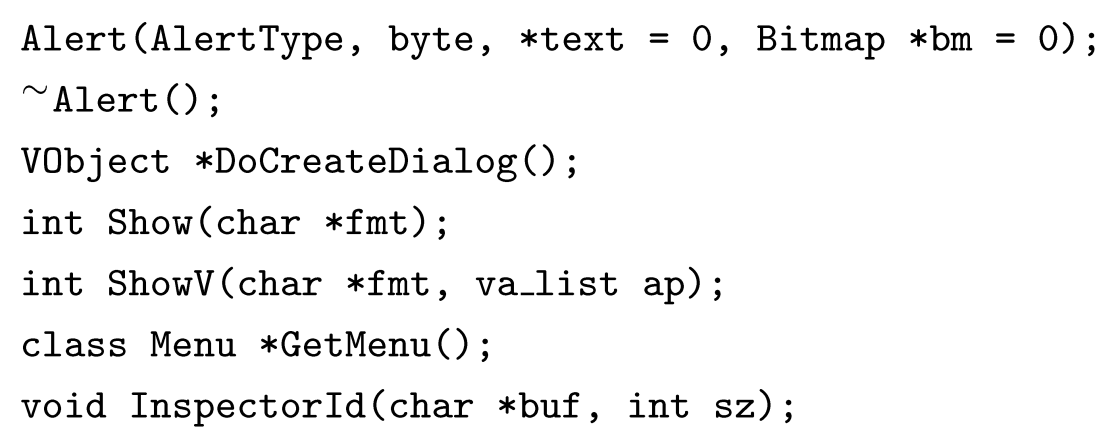
\includegraphics[width=\columnwidth]{nhd-1.png}\par
\(k\) --- total number of methods\par
\(l\) --- total number of types\par
\(\texttt{CAMC} = \frac{1}{k \times l} \times \mathlarger{\sum}_{i=1}^{k} \mathlarger{\sum}_{j=1}^{l} o_{ij}\)\par
\par\columnbreak\par
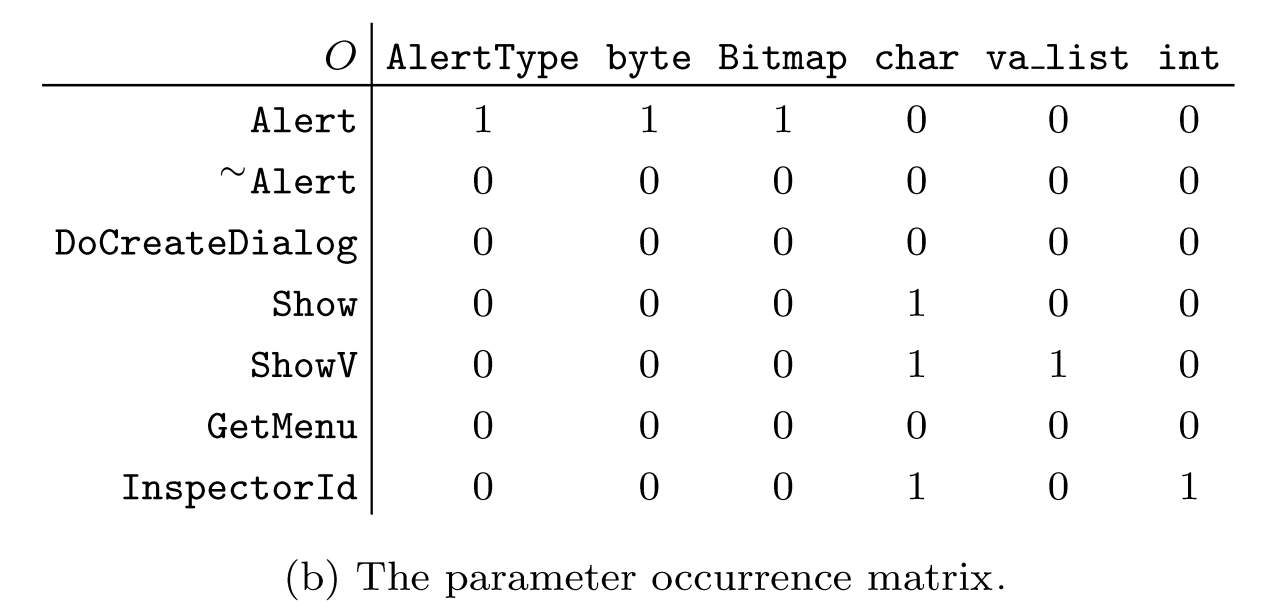
\includegraphics[width=.9\columnwidth]{nhd-2.png}\par
\lnSource{bansiya1999class}
\end{pptWide}}

\lnQuote
  [Steve Counsell]
  {steve-counsell}
  {\textbf{NHD}: The hamming distance (HD) provides a measure of disagreement between rows in a binary matrix. The Normalised Hamming Distance (NHD) metric measures agreement between rows in a binary matrix.}
  {counsell2006interpretation}

\plush{\begin{pptWide}{2}
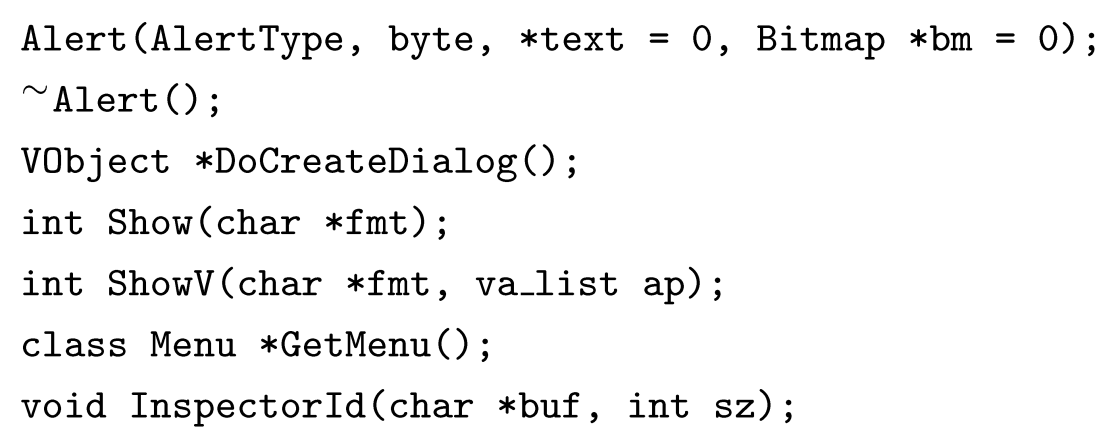
\includegraphics[width=\columnwidth]{nhd-1.png}\par
\(k\) --- total number of methods\par
\(l\) --- total number of types\par
\(\texttt{NHD} = \frac{2}{l \times k \times (k - 1)} \times \mathlarger{\sum}_{j=1}^{k-1} \mathlarger{\sum}_{i=j+1}^{k} a_{ij}\)\par
\par\columnbreak\par
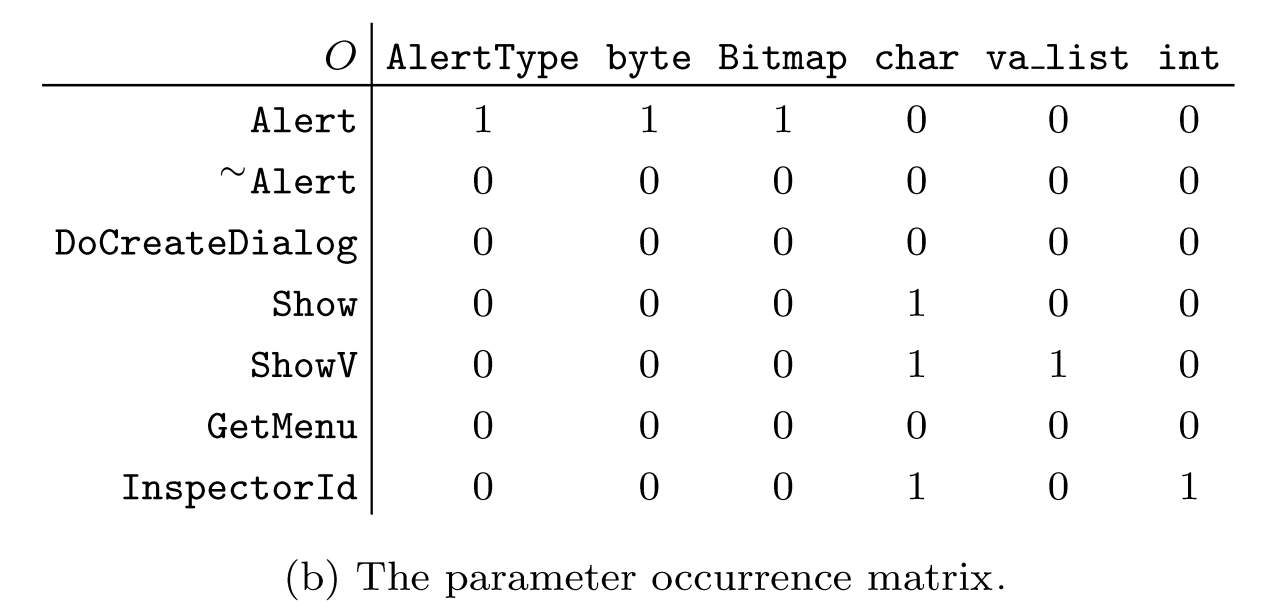
\includegraphics[width=.9\columnwidth]{nhd-2.png}\par
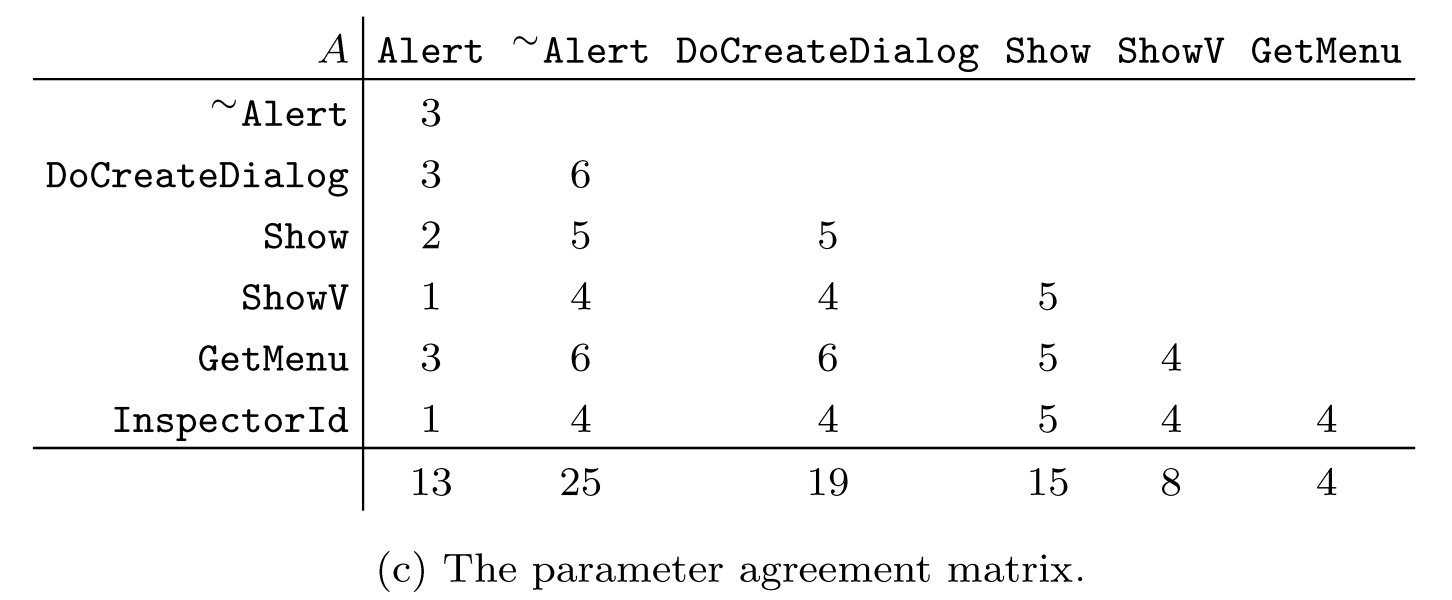
\includegraphics[width=.9\columnwidth]{nhd-3.png}\par
\end{pptWide}}

\lnQuote
  [Robert C. Martin]
  {robert-martin}
  {Classes that have 'fat' interfaces are classes whose interfaces are not \ul{cohesive}. In other words, the interfaces of the class can be broken up into groups of methods.}
  {martin2002}

\pptBanner{InputStream in Java}
\begin{pptWide}{2}
\textcolor{red}{Bad}:
{\scriptsize\begin{ffcode}
abstract class InputStream
  int read();
  int read(byte[] b);
  int read(byte[] b, int o, int l);

class FileInputStream
  implements InputStream
  native int read();
  native int read(byte[] b, int o, int l);
  int read(byte[] b)
    return read(b, 0, b.length);
\end{ffcode}
}
\par\columnbreak\par
\textcolor{green}{Better} (but slower!):
{\scriptsize\begin{ffcode}
interface InputStream {
  int read(byte[] b, int o, int l);

class FileInputStream
  implements InputStream
  native int read(byte[] b, int o, int l);

class OneByteStream
  InputStream s;
  int read()
    byte[] b = new byte[1];
    s.read(b, 0, 1);
    return (int) b[0];
\end{ffcode}
}
\end{pptWide}
\par
\lnSource{bugayenko2016blog0426}
\plush{}


\lnPitch{
\pptBanner{Also Known As...}
\begin{multicols}{2}
\begin{itemize}
  \item ``interface'' in Java
  \item ``protocol'' in Objective-C
  \item ``interface'' in C\#
  \item ``abstract class'' in C++
  \item absent in Python
  \item absent in JavaScript
  \item ``interface'' in Go
  \item ``trait'' in Rust
\end{itemize}\end{multicols}\par
\lnSource{bugayenko2020blog0219}}

\end{document}
